
%\usepackage{enumitem}
\chapter{Analise experimental do desempenho do blockchain  com containers Docker}
\label{chapter_experimento}
% \section{Analise experimental do desempenho do blockchain  com containers Docker}
%         % \textbf{- Estudos de caso}


        \begin{itemize}[label= $\ast$]
            \item \textbf{Estudos de caso}
        \end{itemize}
        % \section{Estudos de caso}

        Nesta seção, foi abordado um estudo de caso com o propósito de simular uma rede blockchain por meio da utilização de containers Docker. O principal objetivo dessa simulação foi explorar as potencialidades e desafios associados à implementação de uma infraestrutura baseada em blockchain em um ambiente de contêineres virtualizados. Ao longo do estudo, foram conduzidas diversas atividades para alcançar uma compreensão aprofundada do funcionamento da rede simulada. Inicialmente, foram configurados e interligados os containers Docker, replicando assim a estrutura distribuída de uma rede blockchain. Esta fase envolveu a criação de nós, a definição de suas interações e a configuração de parâmetros específicos.

        Optei por concentrar a pesquisa no registro de diplomas digitais, apesar das diversas aplicações potenciais para a simulação de Blockchain. Essa decisão estratégica foi motivada pela complexidade e relevância específicas desse cenário, destacando-se, em parte, devido às limitações observadas ao tentar utilizar outros simuladores. Muitas vezes, essas plataformas carecem dos recursos tecnológicos necessários para realizar testes abrangentes e coletar resultados de maneira eficaz.

        Morais (2019) sugere que instituições de ensino possuam a capacidade de emitir diplomas e certificados em formato digital, com a proposta de registrar esses documentos em uma Blockchain para garantir sua autenticidade. Esse conceito envolve a geração de um identificador único para cada documento, que, uma vez registrado na Blockchain, estabelece uma referência permanente. Isso viabiliza a verificação da existência do documento original sempre que necessário.

        
        % Acredito que essa abordagem proporcionará uma compreensão mais aprofundada das implicações práticas da implementação do Blockchain no registro de documentos educacionais digitais, aproveitando ao máximo as vantagens tecnológicas e superando obstáculos anteriores.

        Ao selecionar o registro de diplomas digitais como foco da pesquisa, não apenas busco explorar a eficácia do Blockchain nesse contexto específico, mas também superar as limitações encontradas em outros simuladores.A simulação, desenvolvida em Node.js, cria o bloco gênesis da cadeia e estabelece os nós da Blockchain em containers por meio do Docker. Cada container é equipado com uma imagem Linux que armazena uma réplica dos registros da cadeia de blocos. Após a inicialização, os nós passam a monitorar a validade dos novos blocos adicionados, decidindo se podem ser integrados à rede.\cite{yadav2018performance}
        % Neste estudo, a quantidade de nós a ser instanciada é determinada pelo pesquisador. 
        Inicialmente, optei por simular uma rede com 10 nós, representando um ambiente de pequena escala. Posteriormente, esse número foi aumentado para 20, com o objetivo de observar o comportamento da rede com o dobro de nós. Ao ser executada, a aplicação gera exclusivamente o bloco gênesis, marcando o início da cadeia, e o distribui para todos os nós. A partir desse ponto, os nós monitoram a validade dos novos blocos adicionados, decidindo se eles podem ser integrados à cadeia.

        Os testes foram realizados em um sistema operacional Linux Mint 19.1 de 64 bits. A Figura \ref{Bloco 0} exibe uma representação visual da rede Blockchain gerada pela aplicação, destacando o bloco gênesis da cadeia, o timestamp que indica o momento de sua geração, e o hash de identificação correspondente.

        \begin{figure}[H]
            \centering
            \frame{\includegraphics[width=15cm]{5-analise-experimental/figure/Capture d’écran 2023-12-03 à 18.35.20.png }}
            \caption{Representação grafica do primeiro bloco .}
            \label{Bloco 0}
        \end{figure}


        \begin{itemize}[label= $\ast$]
            \item \textbf{Definição de indicadores de desempenho para análise sistemática}
        \end{itemize}

        Os parâmetros selecionados para análise compreenderam a vazão (throughput), representando a taxa na qual as requisições são atendidas pelo sistema, e o tempo de resposta, que consiste no intervalo decorrido entre o início e a conclusão de um serviço.

        \begin{itemize}[label= $\ast$]
            \item \textbf{Aplicação de cargas de trabalho}
        \end{itemize}

       Para extrair as métricas de vazão e tempo de resposta, conduzimos 30 experimentos. Este número significativo de iterações confere ao experimento uma elevada confiabilidade, aproximando os resultados de uma dinâmica realista. O desvio padrão dos dados experimentais foi de 1,18. Foi aplicado diversas cargas de trabalho, simbolizando distintas quantidades de usuários realizando acessos simultâneos à aplicação. As cargas variaram de 1, 5, 10, 50, 100, 500 e 1000 acessos simultâneos.
       Inicialmente, foi incluido 10 nós na Blockchain e aplicamos várias cargas de trabalho para simular acessos simultâneos à rede. Os testes foram conduzidos em um sistema equipado com um processador Intel Core i5-10210U de 1,60 GHz e 8 GB de memória RAM.
       A ferramenta JMeter possibilita a definição da quantidade de acessos simultâneos. Neste experimento, cada acesso realiza o envio de dados no formato JSON para a aplicação, utilizando o método POST. Esse processo, em um contexto real, simboliza o registro de um diploma digital na cadeia de blocos.

        \begin{itemize}[label= $\ast$]
            \item \textbf{Simulação de Cargas de Trabalho}
        \end{itemize}

        A ferramenta JMeter oferece a capacidade de configurar a quantidade de acessos simultâneos. Neste experimento, cada acesso realiza o envio de dados no formato JSON para a aplicação, utilizando o método POST. Esse procedimento, em um cenário real, representa a inclusão de um diploma digital na cadeia de blocos.

        \begin{itemize}[label= $\ast$]
            \item \textbf{ Resultados }
        \end{itemize}

       Primeiramente, foi realizada uma análise da vazão. O gráfico da Figura \ref{graf_vazao10} ilustra que, à medida que o número de acessos simultâneos aumenta, o valor da vazão tende a se estabilizar. Esse fenômeno ocorreu por volta de 23 requisições por milissegundo, indicando o limite da capacidade de vazão da aplicação.

         \begin{figure}[H]
            \centering
            \frame{\includegraphics[width=15cm]{5-analise-experimental/figure/Capture d’écran 2023-12-03 à 20.33.37.png }}
            \caption{Vazão da Blockchain com 10 nós para diferentes cargas de trabalho.}
            \label{graf_vazao10}
        \end{figure}

        

        Na segunda métrica, levamos em consideração o tempo de resposta. O gráfico apresentado na Figura \ref{graf_tp_resposta} ilustra os resultados obtidos durante o teste com 10 nós. Observa-se no gráfico que, à medida que o número de usuários simultâneos aumenta, o tempo de resposta da aplicação também cresce. Para 1000 acessos simultâneos, o tempo total de resposta atingiu 12845 milissegundos.
        \begin{figure}[H]
            \centering
            \frame{\includegraphics[width=15cm]{5-analise-experimental/figure/Capture d’écran 2023-12-03 à 20.56.01.png }}
            \caption{Tempo de resposta com 10 nós para diferentes cargas de trabalho.}
            \label{graf_tp_resposta}
        \end{figure}

        Em seguida , foi realizado uma simulação da Blockchain com 20 nós para avaliar seu comportamento ao dobrar a quantidade de máquinas conectadas. Uma rede com mais nós oferece maior segurança, tornando mais difícil para um atacante malicioso comprometer a rede, exigindo a alteração de mais de 51% dos nós 

        Focamos na análise do desempenho da Blockchain, considerando vazão e tempo de resposta com o aumento da quantidade de nós conectados. Os resultados indicam que, ao aplicarmos as mesmas cargas de trabalho, a vazão se estabiliza em torno de 23 requisições por milissegundo (Figura \ref{graf_vazao_20}). 
        \begin{figure}[H]
            \centering
            \frame{\includegraphics[width=15cm]{5-analise-experimental/figure/Capture d’écran 2023-12-03 à 21.19.25.png }}
            \caption{Vazão da Blockchain com 20 nós para diferentes cargas de trabalho.}
            \label{graf_vazao_20}
        \end{figure}

        
        Também foi avaliado o tempo de resposta da Blockchain com 20 nós, notando um aumento significativo para todos os casos testados (Figura \ref{graf_tp_resposta_20}).
        \begin{figure}[H]
            \centering
            \frame{\includegraphics[width=15cm]{5-analise-experimental/figure/Capture d’écran 2023-12-03 à 21.24.35.png }}
            \caption{Tempo de resposta com 20 nós para diferentes cargas de trabalho.}
            \label{graf_tp_resposta_20}
        \end{figure}

        
        % Para compreender o motivo da estabilização da vazão em cerca de 23 requisições por 12845 milissegundos, analisamos os percentuais de uso de CPU e memória RAM durante os testes com 1000 requisições simultâneas. Utilizamos o plugin Perfmon3 adicionado ao JMeter para observar essas métricas.

       \begin{itemize}[label= $\ast$]
            \item \textbf{Considerações Finais}
        \end{itemize}
        
        Este estudo abordou a simulação de uma rede Blockchain por meio de containers Docker e apresentou uma metodologia bem definida para avaliação de desempenho em sistemas baseados em Blockchain. A pesquisa envolveu a variação na quantidade de nós na Blockchain, examinando cenários com 10 e 20 nós, e aplicando diferentes cargas de trabalho para avaliação do desempenho. Utilizando a ferramenta JMeter, as métricas de vazão e tempo de resposta foram consideradas nos testes.

Os resultados destacaram que a Blockchain com 20 nós apresentou um tempo de resposta 70\% maior em comparação com a configuração anterior, indicando que, embora o uso de Blockchain proporcione maior segurança, pode ocorrer uma redução no desempenho da aplicação. Isso sublinha a importância de equilibrar segurança e desempenho ao projetar sistemas baseados em Blockchain. A utilização de simulações possibilita avaliar o comportamento da aplicação antes da implementação, permitindo uma análise prévia do seu desempenho.

    %     YCSB (Yahoo Cloud Serving Benchmark): O YCSB é uma ferramenta de benchmark amplamente utilizada para avaliar o desempenho de sistemas de armazenamento e bancos de dados, incluindo sistemas de banco de dados NoSQL. Ele permite medir a capacidade de um sistema de processar cargas de trabalho de leitura e gravação de dados em uma ampla gama de cenários. Isso ajuda a determinar como um sistema se comporta sob diferentes condições de uso, como o número de operações por segundo, latência e escalabilidade.
        
    %     Smallbank: Smallbank é outro benchmark projetado para medir o desempenho de sistemas de gerenciamento de bancos de dados em cenários de processamento de transações. Ele simula um conjunto de operações bancárias comuns, como saques, depósitos e transferências, e avalia como um sistema lida com essas transações em termos de taxa de transferência, latência e eficiência.

    %     \begin{itemize}[label= $\blacklozenge$]
    %         \item \textbf{Throughput and latency(Taxa de transferência e latência):} 
    %         Foi avaliado o desempenho máximo dos três sistemas usando 8 servidores e 8 clientes simultâneos durante um período de 5 minutos. Cada cliente enviou transações para um servidor com uma taxa variando de 8 tx/s a 1024 tx/s. Os resultados demonstram que o Hyperledger supera outros sistemas em termos de taxa de transferência, com um desempenho até 5,5 vezes maior que o Ethereum e 28 vezes maior que o Parity. Figure \ref{Blockchain performance}

    %         A diferença entre o desempenho do Hyperledger e Ethereum se deve ao protocolo de consenso, sendo o primeiro baseado no PBFT (Practical Byzantine Fault Tolerance) e o segundo no PoW (Proof of Work). Com 8 servidores, o custo de comunicação na transmissão de mensagens no Hyperledger é significativamente mais eficiente do que a mineração de blocos, que possui uma dificuldade ajustada para cerca de 2,5 segundos por bloco.Figure \ref{Blockchain performance}.b
    % \begin{figure}[H]
    %         \centering
    %         \frame{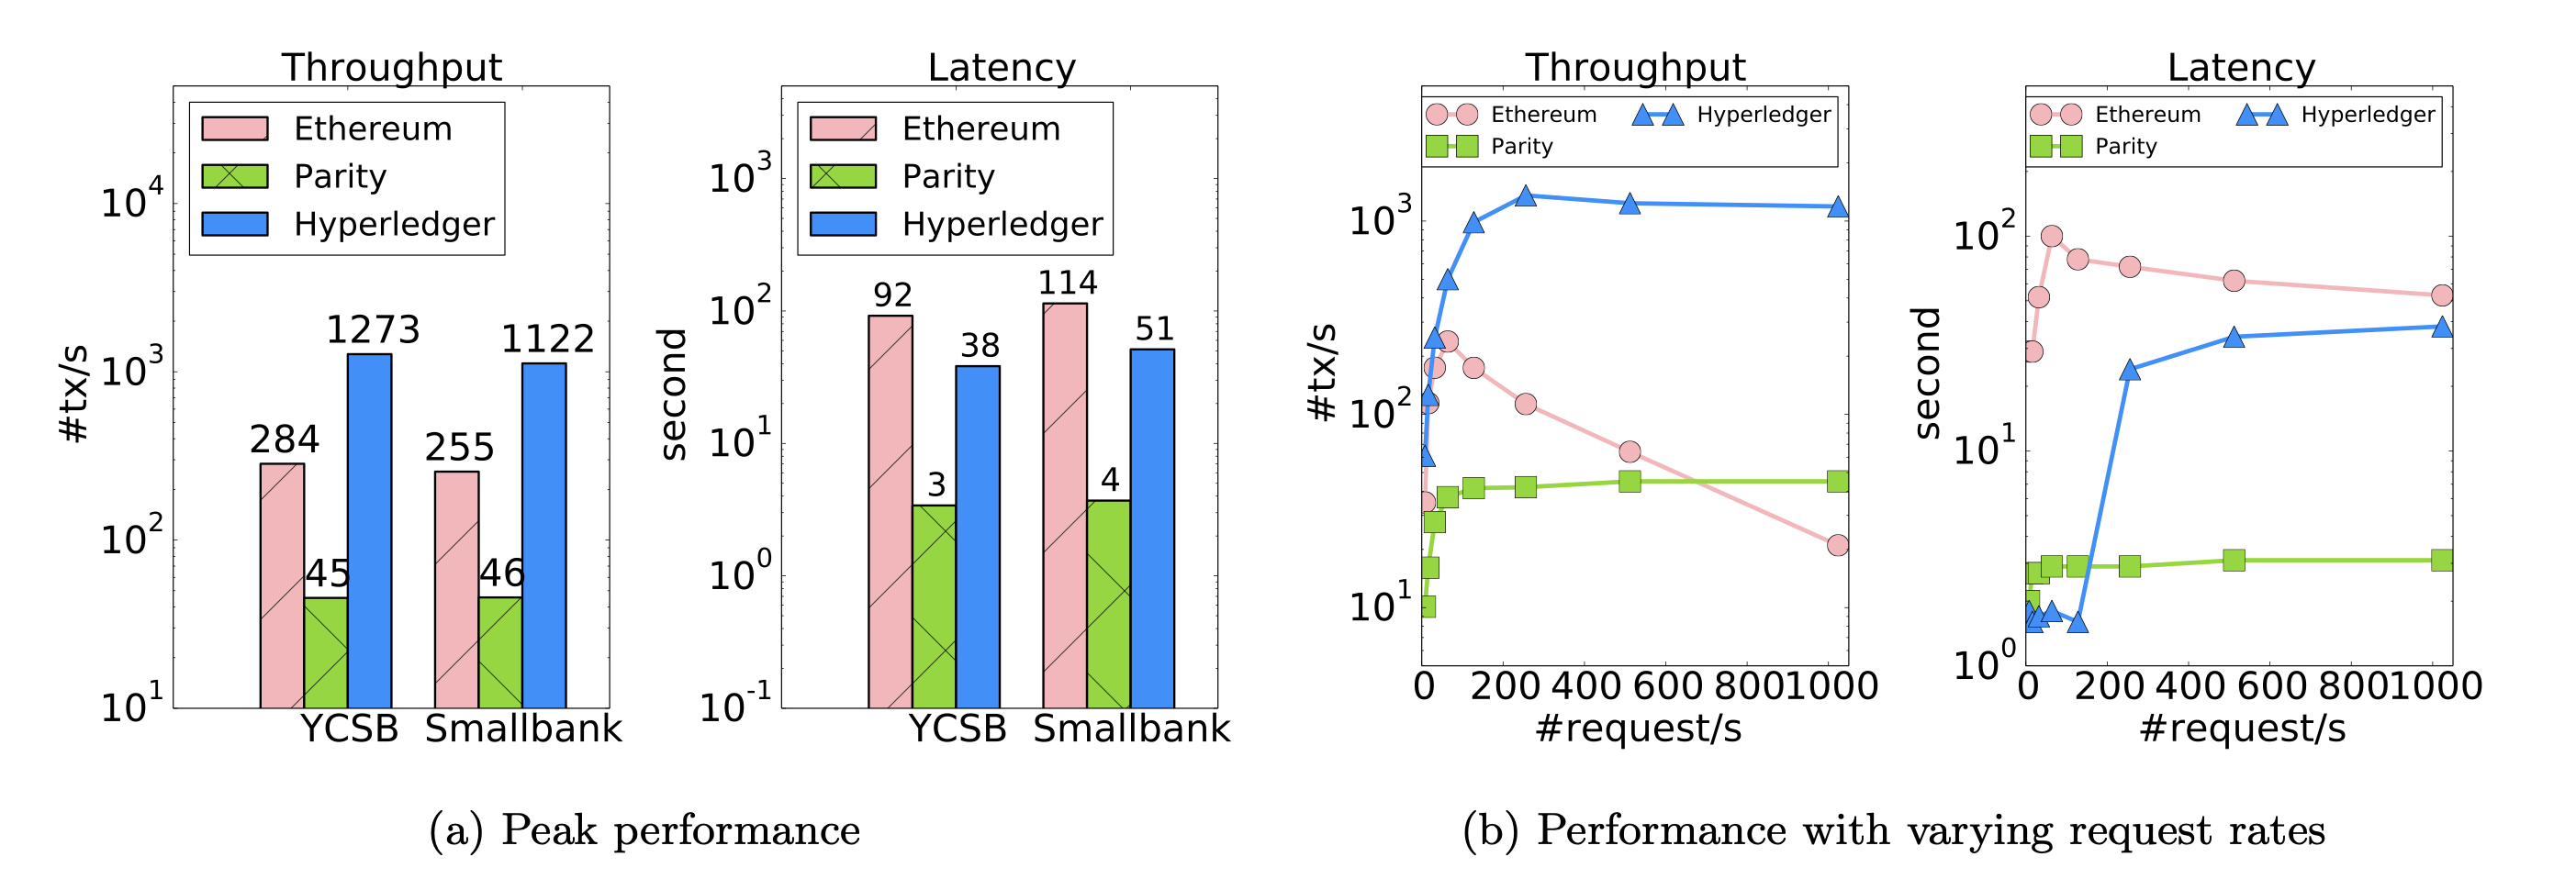
\includegraphics[width=15cm]{4-Analise-de-desempenho-do-Blockchain/figure/Blockchain-perfomance.png}}
    %         \caption{Blockchain performance with 8 clients and 8 servers. \cite{blockbench}, .}
    %         \label{Blockchain performance}
    %     \end{figure}

    %         A Figura \ref{clients request} compara os tamanhos da fila antes e depois de os sistemas atingirem seu pico de taxa de transferência. Com apenas 8 tx/s, as filas do Ethereum e Hyperledger permanecem em tamanhos aproximadamente constantes, mas o tamanho da fila do Parity aumenta com o tempo. Mais interessante ainda, sob cargas elevadas (512 tx/s por cliente), a fila do Parity é sempre menor do que a do Ethereum e do Hyperledger.
    %         O desempenho do Parity, por sua vez, não é afetado pelo protocolo de consenso, visto que o PoA (Proof of Authority) é esperado como mais eficiente. O Parity mantém uma taxa de transferência e latência constantes, mesmo sob cargas elevadas. Isso sugere que o Parity processa transações a uma taxa constante e impõe um limite máximo na taxa de solicitação de clientes, obtendo, assim, uma menor taxa de transferência e latência em comparação com outros sistemas.

    %         \begin{figure}[H]
    %             \centering
    %             \frame{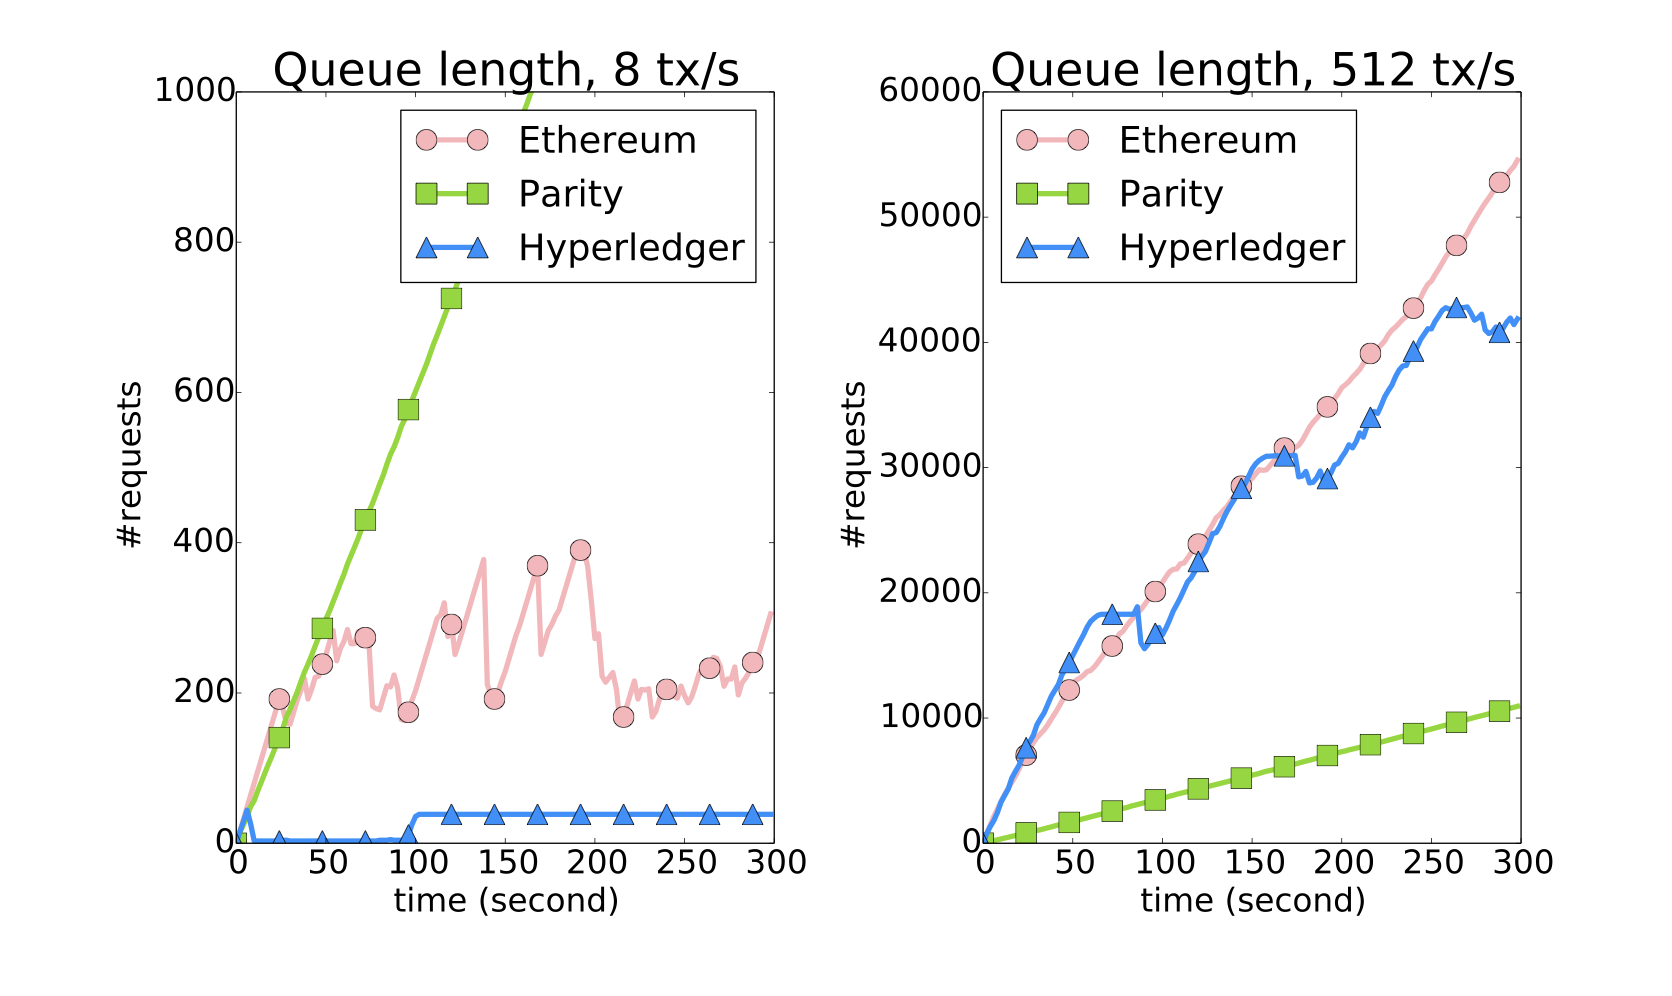
\includegraphics[width=15cm]{4-Analise-de-desempenho-do-Blockchain/figure/Clients request.png}}
    %             \caption{Client’s request queue, for request rates of 8 tx/s and 512 tx/s \cite{blockbench}, .}
    %             \label{clients request}
    %         \end{figure}

    %         Além disso, foram observadas diferenças nas cargas de trabalho YCSB e Smallbank, resultando em uma redução de 10\% na taxa de transferência e um aumento de 20\% na latência. Isso ocorre porque a execução de contratos inteligentes Smallbank é mais onerosa, envolvendo mais leituras e gravações nos estados do blockchain.

    %         No pico de sua taxa de transferência, o Hyperledger gera 3,1 blocos por segundo e atinge uma taxa de transferência total de 1273 tx/s, embora ainda seja menor do que a de sistemas de banco de dados em memória. Os resultados também demonstram que, com o aumento do tamanho dos blocos, a taxa de geração de blocos diminui proporcionalmente, sem melhoria na taxa de transferência global.
    %     \end{itemize}
        

       
